\subsection{Understand Model Behaviors}
\begin{figure}[t]
	\centering
	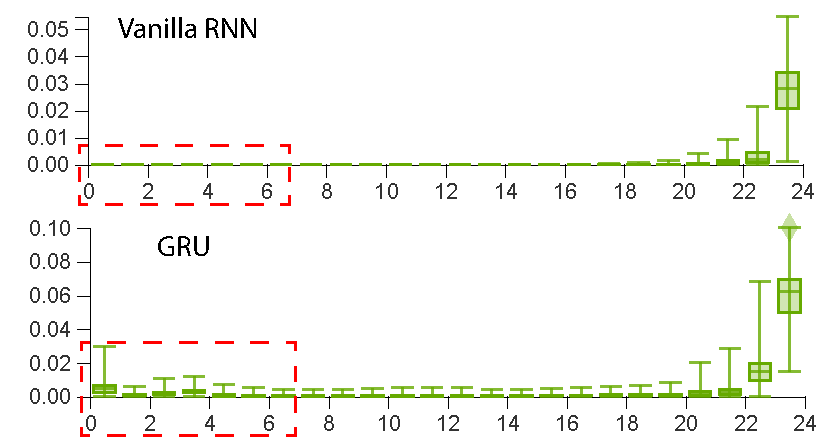
\includegraphics[width=0.40\textwidth]{pictures/Evaluation/FI_comparison.pdf}
	\vspace{-3mm}
	\caption{Compare the temporal importance of \textit{100\_NE\_PM25}  across different models. 
% 	The dashed rectangle show both GRU has a "tail" while vanilla RNN does not.
	}
	\label{fig:gru_vs_rnn}
	\vspace{-4mm}
\end{figure}

\subsubsection{Model Mechanism}
This case study is conducted to understand what RNN models learn and to compare different models trained for air pollutant forecasting. 
With MultiRNNExplorer, we are able to select models at any epoch. Fig.~\ref{fig:teaser}A shows the Cluster View of GRU-Dense; by observing the cluster of features, we find that the features with same feature types are likely to cluster together such as the \textit{\color{RHColor}{Relative Humidity}} and \textit{\color{DPColor}{Dew-point}}, are exactly grouped into two separated clusters shown as Fig.~\ref{fig:teaser}A$_4$.
Moreover, we find that the $\color{PM25Color}{PM_{2.5}}$ and $\color{PM10Color}{PM_{10}}$ are always clustered together as shown in Fig.~\ref{fig:teaser}A$_1$ and Fig.~\ref{fig:teaser}A$_2$.
The domain expert explains that $\color{PM25Color}{PM_{2.5}}$ and $\color{PM10Color}{PM_{10}}$ are highly correlated because they are always generated together.
% On the other hand, we notice that all the features on \color{PM25Color}{$PM_{2.5}$} and \color{PM10Color}{$PM_{10}$} are also grouped by the distance: Fig. \ref{fig:teaser}A$_1$ and A$_2$ show that the features far away from (200km and 300km) or nearby (closer than 30km) the target location are clustered in different groups. 
This  shows that the model GRU-Dense is able to learn the information related to spatial locations.  

% Another thing of interest is the hyper-parameters of the model such as the RNN size. 
% \yh{How the hidden unit size relates with the observation below?}
% In the cluster view, we notice that a cluster of hidden units have very weak relationship to feature clustersi(Fig. \ref{fig:teaser} a4. \QM{explain?}.
% Such pattern also appears in the exploration of other models.

\begin{figure}[t]
	\centering
	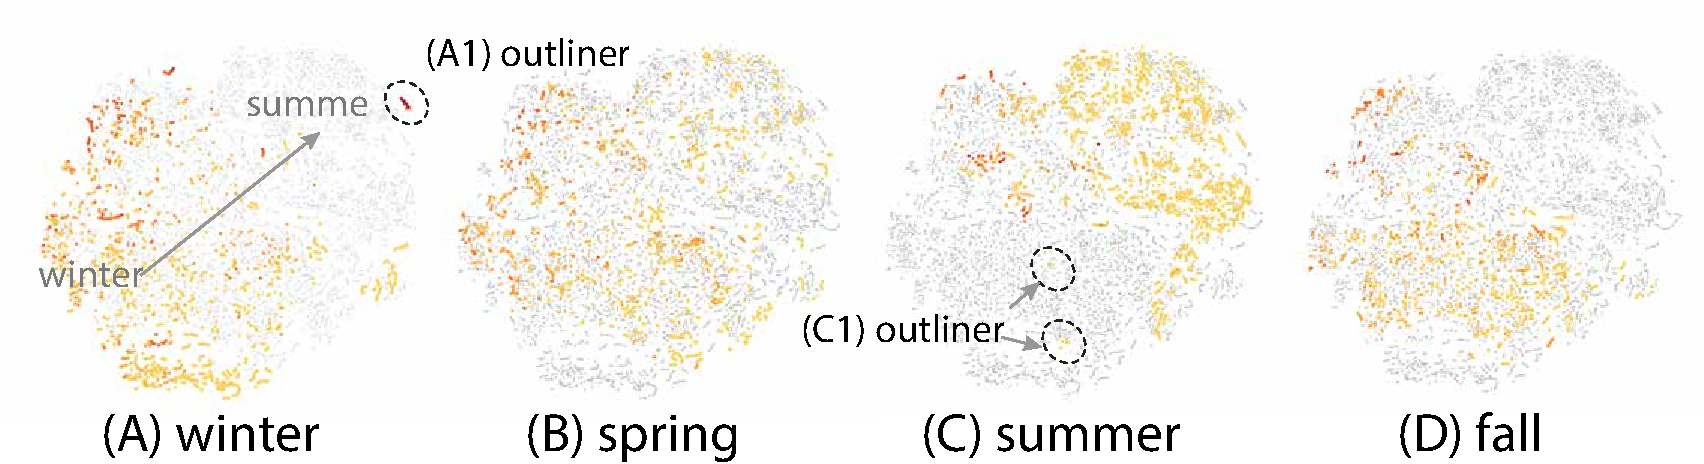
\includegraphics[width=0.45\textwidth]{pictures/Evaluation/seasonal_behavior.pdf}
	\vspace{-3mm}
	\caption{Projection View across four seasons whose time range are defined by local standards.}
	\label{fig:seasonal_feature}
	\vspace{-4mm}
\end{figure}

\subsubsection{Feature importance}
We select the individual sequences of Fig.~\ref{fig:teaser}D$_2$ and re-sort the features by the importance. 
From the Feature Importance View, the top important features are listed as Fig.~\ref{fig:teaser}C, and we observe that most of them are related to feature $\color{SO2Color}{SO_{2}}$ and \textit{\color{WINDColor}{Wind Speed}}.
Then, top features change to $\color{SO2Color}{SO_2}$ and $\color{PM25Color}{PM_{2.5}}$ in later epochs. 
This observation shows that feature importance may vary across different individual cases. 
By default without selecting any sequences, the features are ranked according to their average importance over of all the test cases. 
We find that the \textit{\color{WINDColor}{Wind Speed}} is a major factor that influences the forecast because the wind related features are ranked in front.
% ~\yh{how? larger wind speed indicates higher predicted value?}. 
The domain experts point out that as there are very few factories in Hong Kong, the local emissions are not a major reason that influences the forecast result. 
Instead, the $PM$ pollutants are easily transported from the north, west, and east of mainland China, thus the $wind$ plays an important role in the forecast of $\color{PM25Color}{PM_{2.5}}$ and $\color{PM10Color}{PM_{10}}$.
% 0.76
% \begin{figure*}[ht]
% 	\centering
% 	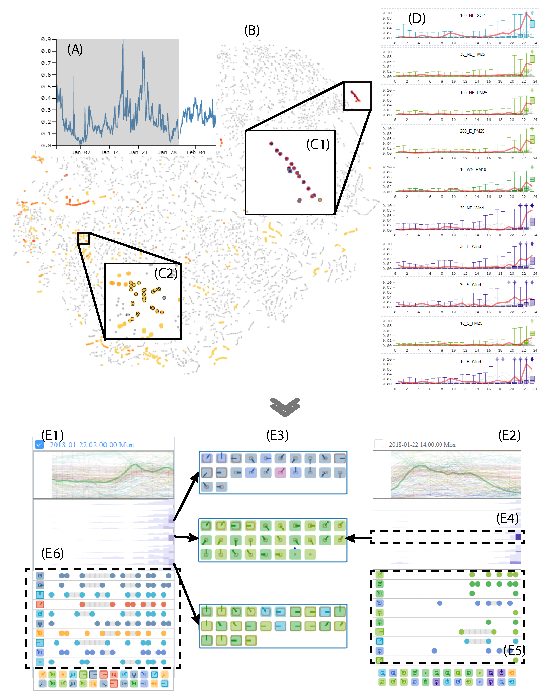
\includegraphics[width=1\textwidth]{pictures/Evaluation/winter_exploration.pdf}
% 	\vspace{-3mm}
% 	\caption{
% 	Case exploration for the $PM_{2.5}$ forecast in winter. A, B) Filter and highlight the individual cases in January 2018; C1, C2) Two groups of individual cases are selected by brushing; D) The top 10 importance features for the group selected in C1; E1, E2) Representative cases of C1 and C2.}
% 	\label{fig:winter_exploration}
% 	\vspace{-4mm}
% \end{figure*}

\begin{figure}[t]
	\centering
	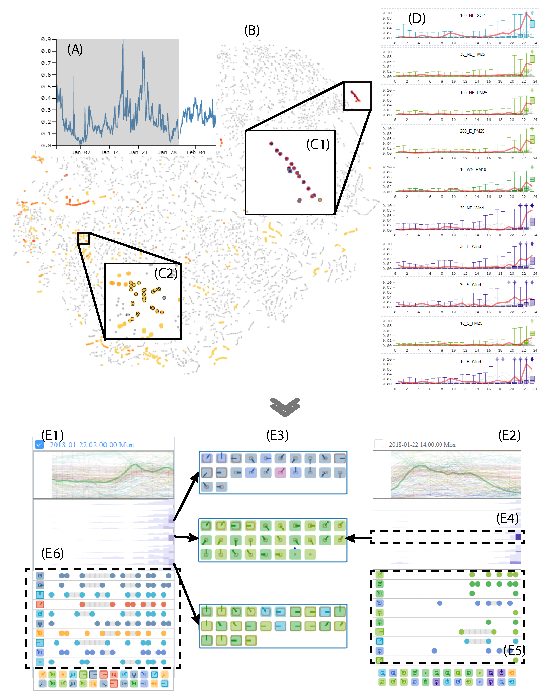
\includegraphics[width=0.45\textwidth]{pictures/Evaluation/winter_exploration.pdf}
	\vspace{-3mm}
	\caption{Case exploration for the $PM_{2.5}$ forecast in winter. A, B) Filter and highlight the individual cases in January 2018; C1, C2) Two groups of individual cases are selected by brushing; D) The top 10 importance features for the group selected in C1; E1, E2) Representative cases of C1 and C2.}
	\label{fig:winter_exploration}
	\vspace{-4mm}
\end{figure}
During the exploration of different models, we notice that the temporal pattern of the Feature Importance View is very different across different models. 
Fig.~\ref{fig:gru_vs_rnn} compares the feature importance for vanilla RNN and GRU.
With the selected feature of \textit{100\_NE\_PM25}, one observation is that the Feature Importance Views of model GRU has a ``tail" (Fig.~\ref{fig:gru_vs_rnn}) especially for the first three timestamps, which is not observed in vanilla RNN.
% While the corresponding feature for vallina RNN have no such kind of pattern. 
This solves one question raised by the domain experts: is it necessary to use such complex models like RNN to conduct air pollutant forecasting tasks?
It is a controversial question~\cite{brownlee2017long} as in some applications all important information is included within within recent small time ranges~\cite{gers2002applying} and do not necessarily require complex machine learning models. 
By using our system, we can find that the GRUs are able to memorize more long-term information than vanilla RNNs. 
Since the air pollutant and meteorology features (such as temperature) have a daily periodic pattern, the input features around 24 hours ahead are also considered relevant to the forecast. 
In addition, since the GRU model have better performance compared with vanilla RNNs from Table~\ref{table:model_configuration}. 
% ~\yh{requires some logic to connect to gated RNN.}
We think the gate RNNs are applicable for the air pollutant forecast. 

